\documentclass[10pt,twocolumn]{article}

\usepackage[margin=0.75in,columnsep=0.25in]{geometry}
\usepackage{amsmath,amssymb}
\usepackage{booktabs}
\usepackage{graphicx}
\usepackage{float}
\usepackage[hidelinks]{hyperref}
\usepackage{xcolor}
\usepackage{natbib}
\usepackage{caption}
\usepackage{microtype}
\captionsetup{font=small,labelfont=bf}
\graphicspath{{../results/figures/}}
\setlength{\parskip}{0.2em}

\newcommand{\tab}[1]{\input{../results/tables/#1.tex}}

\title{\vspace{-1.2em}Tabular Q-Learning versus Deep Q-Networks:\\ Sample Efficiency, Sparse Rewards and DQN Ablations}
\author{Aispur Santiago \quad Amaya Bryan\\[0.2em]
\small Intelligent Agents --- Instructor: PhD Armas Rolando}
\date{\today}

\begin{document}
\maketitle

%% RESULTS-DEPENDENT TEXT IS FILLED IN AFTER THE EXPERIMENTS FINISH
\begin{abstract}
We compare tabular Q-learning on a discretized state space with a Deep Q-Network (DQN) implemented
from scratch in PyTorch. Every curve is indexed by \emph{cumulative environment steps}, averaged over
ten fixed seeds with 95\% Student-$t$ confidence bands, and evaluated greedily ($\varepsilon=0$, frozen
weights) at regular checkpoints. On CartPole-v1, DQN reaches the solved threshold in
$\approx$7$\times$ fewer environment steps than the best tabular agent, but each step costs
$\approx$23$\times$ more CPU, so tabular learning is $\approx$3$\times$ cheaper per unit of \emph{compute}. On the
sparse-reward MountainCar-v0, DQN with $\varepsilon$-greedy exploration never reaches the goal and
converges to a flat $Q\approx-1/(1-\gamma)$. An optimistically initialized table solves it, while a
pessimistically initialized one fails like DQN, which isolates optimism as the cause. On LunarLander-v3,
ablations show how the target network and the replay buffer each contribute to stability. We close
with an analysis of why neither family scales to continuous control or pixel observations.
\end{abstract}

\section{Introduction}
The question we study is not only \emph{whether} an agent learns, but \emph{why} it wins or loses
under a fair experimental protocol. We hold three rules throughout. (i) Algorithms are compared on
environment steps, because a tabular agent's early CartPole episodes last $\sim$20 steps while a good
DQN episode lasts 500, so an ``episode'' axis is not a common clock. (ii) Performance is measured by
periodic greedy evaluation with frozen weights, reported separately from the noisy $\varepsilon$-greedy
training returns. (iii) Every configuration uses ten seeds, with seeding of
\texttt{random}, NumPy, \texttt{torch.manual\_seed} and \texttt{env.reset(seed=\dots)}. Negative results
are reported and diagnosed rather than tuned away. All code, raw logs, weights and the command that
regenerates every figure (\texttt{python experiments/run\_all.py}) are in the accompanying repository.

\section{Background}
\paragraph{Tabular Q-learning.} An off-policy TD control method \citep[Sec.~6.5]{sutton2018}:
\begin{equation}
Q(s,a)\leftarrow Q(s,a)+\alpha\big[r+\gamma\max_{a'}Q(s',a')-Q(s,a)\big].
\label{eq:q}
\end{equation}
Continuous observations must first be mapped to a finite index by binning each dimension
(Sec.~\ref{sec:setup}). The bootstrap term is dropped only on a \emph{true} terminal transition.
A time-limit truncation is not terminal, so we still bootstrap there.

\paragraph{DQN.} \citet{mnih2015} replace the table with a network $Q_\theta(s,\cdot)$ that outputs one
value per action and minimise a Huber loss between $Q_\theta(s,a)$ and the target
$y=r+\gamma(1-d)\max_{a'}Q_{\bar\theta}(s',a')$. Two mechanisms make this stable. An \emph{experience
replay} buffer is sampled uniformly, which breaks the temporal correlation of consecutive transitions and
reuses data. A \emph{target network} $\bar\theta$ is copied from $\theta$ only every $C$ steps, so the
regression target does not move with every gradient step. In code, $Q_\theta(s,a)$ for the actions
actually taken is extracted with \texttt{q(s).gather(1, a)}; the $\max$ is used only for the next-state target.

\paragraph{Extensions.} \emph{Double DQN} \citep{vanhasselt2016} decouples action selection from evaluation:
$y=r+\gamma Q_{\bar\theta}(s',\arg\max_{a'}Q_\theta(s',a'))$, which reduces the overestimation bias of $\max$.
\emph{Dueling DQN} \citep{wang2016} decomposes $Q(s,a)=V(s)+A(s,a)-\tfrac{1}{|\mathcal A|}\sum_{a'}A(s,a')$.

\section{Experimental setup}
\label{sec:setup}
\paragraph{Environments.} Gymnasium 1.3 \citep{towers2024gymnasium}: CartPole-v1 (4-D state,
2 actions, +1 per step, truncated at 500, solved at 475), MountainCar-v0 (2-D, 3 actions, $-1$ per step,
truncated at 200) and LunarLander-v3 (8-D, 4 actions, shaped reward, solved at 200).

\paragraph{Discretization.} Each dimension is split into $k$ uniform bins between a lower and an upper
bound. Values beyond the bounds fall into the outer bins. Position ($\pm2.4$) and pole angle
($\pm0.2095$\,rad $=12^\circ$) use the termination limits as bounds. The velocities are unbounded in the
observation space, so we \emph{clip} them at $\pm3.0$ and $\pm3.5$. Table~\ref{tab:t1_obs_ranges}
justifies this: over 50k steps under a random policy and under the trained DQN, the largest observed
values are 2.83 (cart velocity) and 2.92 (angular velocity), so no visited value exceeds the bounds and
almost no bin is wasted on states that never occur. We also support hand-made boundaries per dimension,
which we use to study the pole angle.

\begin{table}[t]
\centering\small
\caption{Hyper-parameters. Only the switch named in each configuration changes.}
\label{tab:hparams}
\resizebox{\columnwidth}{!}{%
\begin{tabular}{lll}
\toprule
 & CartPole / MountainCar & LunarLander \\
\midrule
Tabular $\alpha,\gamma$ & 0.1, 0.99 & -- \\
Tabular $\varepsilon$ & $1\!\to\!0.01$ over 500k (CP); MC: as DQN & -- \\
DQN net & 4/2$\to$128$\to$128 & 8$\to$256$\to$256 \\
Optimiser & Adam, lr $5\!\cdot\!10^{-4}$ & Adam, lr $5\!\cdot\!10^{-4}$ \\
Batch / buffer & 64 / 50k & 128 / 100k \\
Learning starts & 1k & 10k \\
Train freq. & every step & every 4 steps \\
Target update & hard, every 500 & hard, every 1000 \\
DQN $\varepsilon$ & $1\!\to\!0.05$ over 25k (MC: 30k) & $1\!\to\!0.05$ over 100k \\
Loss / grad clip & Huber / 10 & Huber / 10 \\
Budget & CP: 1M tab., 200k DQN; MC: 500k & 500k \\
Evaluation & 10 ep. every 5k & 10 ep. every 10k \\
\bottomrule
\end{tabular}}
\end{table}

\paragraph{Protocol and statistics.} Hyper-parameters are in Table~\ref{tab:hparams}. At each checkpoint
we run 10 greedy episodes on a separate environment, from the same evaluation seeds at every checkpoint,
so that changes in the curve reflect the policy rather than the sampled start states. We report the
mean over 10 seeds with a 95\% Student-$t$ interval ($t_{9,0.975}=2.26$, deliberately wider than the
normal 1.96). Plotted greedy curves use a short trailing average over checkpoints (5 for CartPole, 3
elsewhere), applied per seed before aggregation; the tables use raw values. Summary metrics, computed
per seed: \emph{final} (mean of the last 3 checkpoints), \emph{best}, \emph{AUC} (mean over all
checkpoints, which rewards speed and stability), \emph{drop} = best $-$ final (forgetting) and steps to
threshold. Every run uses one CPU thread. Seeds 0--4 (and 8--9 for LunarLander) ran on a laptop
(Ryzen 5 7235HS) and the others on 4-vCPU GitHub Codespaces with identical pinned packages. Learning
metrics use all seeds, and CPU-time figures use only the laptop runs so that timings come from one CPU.

\tab{t1_obs_ranges}

\section{Tier 1: tabular Q-learning vs.\ DQN}
\subsection{CartPole-v1}
\label{sec:cp}

\begin{figure*}[t]
\centering
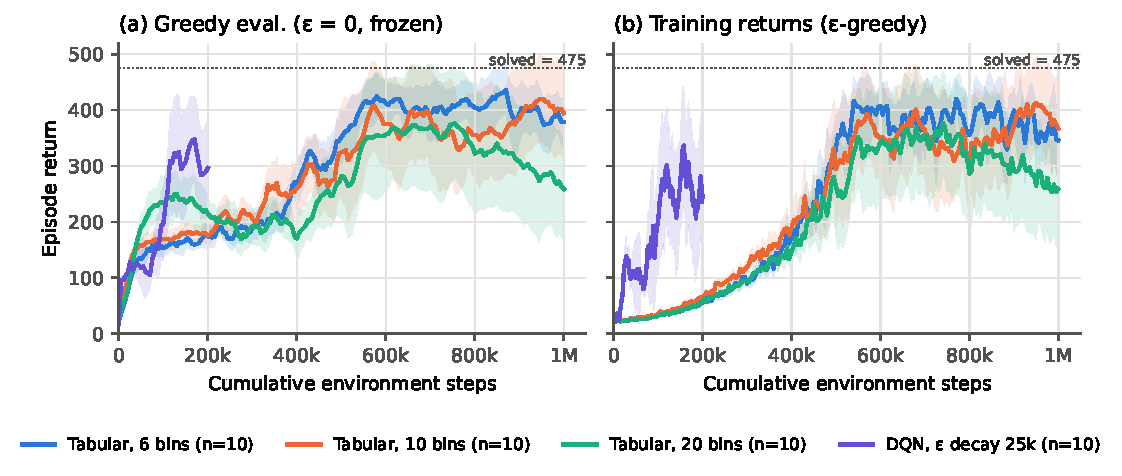
\includegraphics[width=0.92\textwidth]{t1_tabular_vs_dqn.pdf}
\caption{CartPole-v1 on a common x-axis of environment steps. (a) Greedy evaluation; (b) training returns
(20-episode moving average). DQN (200k budget) rises within the first $\sim$100k steps, while the tables
need $\sim$400--550k. Bands: 95\% CI over 10 seeds; greedy curves smoothed over 5 checkpoints.}
\label{fig:t1}
\end{figure*}

\tab{t1_cartpole}

\paragraph{Sample efficiency.} Fig.~\ref{fig:t1} and Table~\ref{tab:t1_cartpole} show the core trade-off.
With the best decay schedule, DQN first reaches a greedy return $\ge$475 after $56\pm16$k environment steps
(10/10 seeds). The fastest table (10 bins) needs $382\pm58$k, so DQN is $\approx$6.9$\times$ more
sample-efficient. At an \emph{equal} budget of 200k steps, DQN ($\varepsilon$ decay 5k) scores $356\pm95$
against $175$--$215$ for the three tables (Welch $t=4.2$, $p=0.002$ vs.\ 10 bins). The mechanism is
generalization: a gradient step on one state also moves $Q$ at nearby states, whereas a table cell learns
only from its own visits.

\paragraph{Compute.} The comparison reverses on CPU time. Measured on the same laptop, a tabular step costs
0.097\,ms and a DQN step 2.24\,ms (a forward pass to act plus a backward pass on a 64-sample batch), a factor
of 23. Reaching 475 therefore costs $\approx$37 CPU-seconds for the table and $\approx$124 for DQN:
tabular learning is 3.4$\times$ cheaper in \emph{compute}. DQN is sample-efficient but compute-hungry,
and tabular Q-learning is the reverse. Which one is ``faster'' depends on whether environment interaction
or computation is the scarce resource.

\paragraph{Number of bins.} More bins do not monotonically help. Six bins (1{,}296 states) visit 39\% of the
table, ten bins (10{,}000) 18\%, and twenty bins (160{,}000) only 4.6\%. Ten bins is the best compromise.
It is the fastest to the threshold ($382\pm58$k steps, 10/10 seeds) and has the highest final score
($392\pm81$). Twenty bins is the worst on every metric: final $263\pm96$, only 7/10 seeds ever reach 475,
the largest drop after the peak ($212\pm88$) and the largest seed-to-seed spread. Six bins learns
reliably (10/10) but more slowly ($518\pm59$k), because it cannot represent the policy as precisely. The
difference between 6 and 20 bins in final score is suggestive but not significant at 5\% ($p=0.07$), so
we state it as a trend. The mechanism is the classic bias--variance trade-off of state aggregation:
coarse cells generalize ``for free'' but cap precision, and fine cells are precise but data-starved.
After 1M steps (\,$\approx$10k episodes) 95\% of the 20-bin table has never been updated.

\paragraph{Pole-angle boundaries.} Fig.~\ref{fig:angle} fixes the other dimensions at 10 bins and changes
only the angle bins. With two angle bins (only the \emph{sign} of the tilt) the agent cannot tell a slight
tilt from a dangerous one. Over the first 200k steps it averages $107\pm8$ against $165\pm14$ for 10 uniform
bins (Welch $p<10^{-6}$), and its AUC is the lowest ($226$ vs.\ $294$). Putting 10 bins inside
$|\theta|<0.1$\,rad, where the pole spends nearly all its time, learns more slowly at first ($120\pm10$)
because the fine cells need more visits, and ends level with uniform binning (final $362$ vs.\ $392$,
CIs overlap). Resolution only pays off where the agent has enough data to fill it.

\begin{figure}[t]
\centering
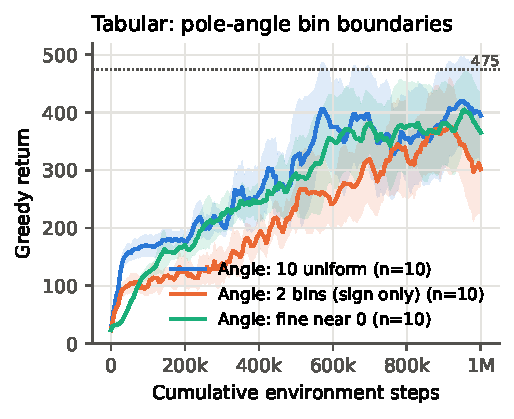
\includegraphics[width=\columnwidth]{t1_angle_boundaries.pdf}
\caption{Tabular CartPole: only the pole-angle boundaries change; all other dimensions use 10 bins.}
\label{fig:angle}
\end{figure}

\paragraph{$\varepsilon$-decay and forgetting.} Fig.~\ref{fig:eps} varies only the length of the linear
$\varepsilon$ decay. On CartPole, fast decay (5k steps) is best both early (mean greedy return $190\pm52$
over the first 50k steps) and late ($379\pm48$ after 150k), and 10/10 seeds reach 475. CartPole needs little
exploration: random actions already visit the relevant near-upright states, so the sooner the agent
exploits, the sooner its data comes from good trajectories. Slow decay (100k) spends half the budget
acting mostly at random. Its training returns stay low until $\varepsilon$ is small, and only 2/10 seeds
reach 475 within 200k steps. Every fast- and medium-decay seed (20/20) also shows \emph{catastrophic
forgetting}: the greedy return reaches $\ge$475 and later falls below 200, with mean drops of 160--200.
Once the policy is good, the 50k-transition buffer fills with near-upright states only, and the
network overwrites what it knew about recovering from large tilts. This is why performance must be
tracked \emph{during} training rather than only at the end: a final-checkpoint evaluation alone would
report $340\pm134$ for a method that had already solved the task.

\begin{figure*}[t]
\centering
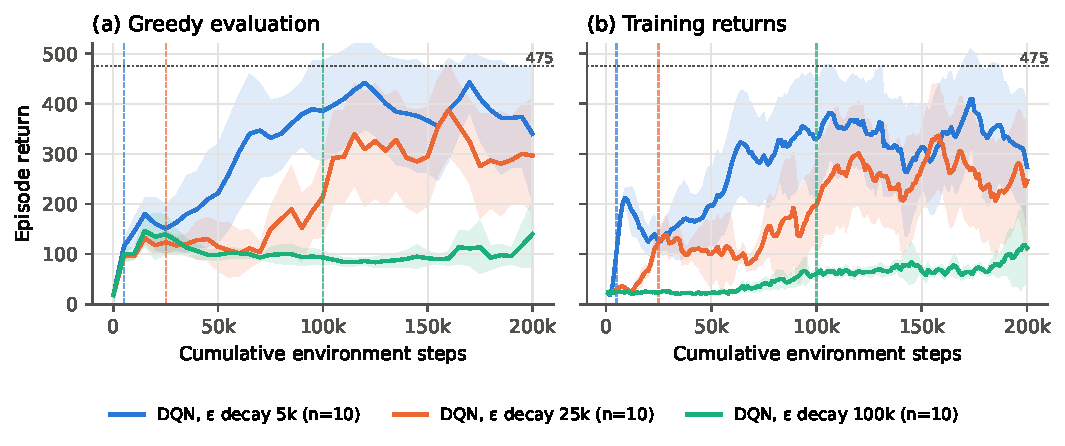
\includegraphics[width=0.92\textwidth]{t1_dqn_eps_decay.pdf}
\caption{DQN on CartPole with three linear $\varepsilon$-decay lengths (dashed lines mark the end of each decay).}
\label{fig:eps}
\end{figure*}

\subsection{MountainCar-v0: a planned negative result}
\label{sec:mc}
\begin{figure*}[t]
\centering
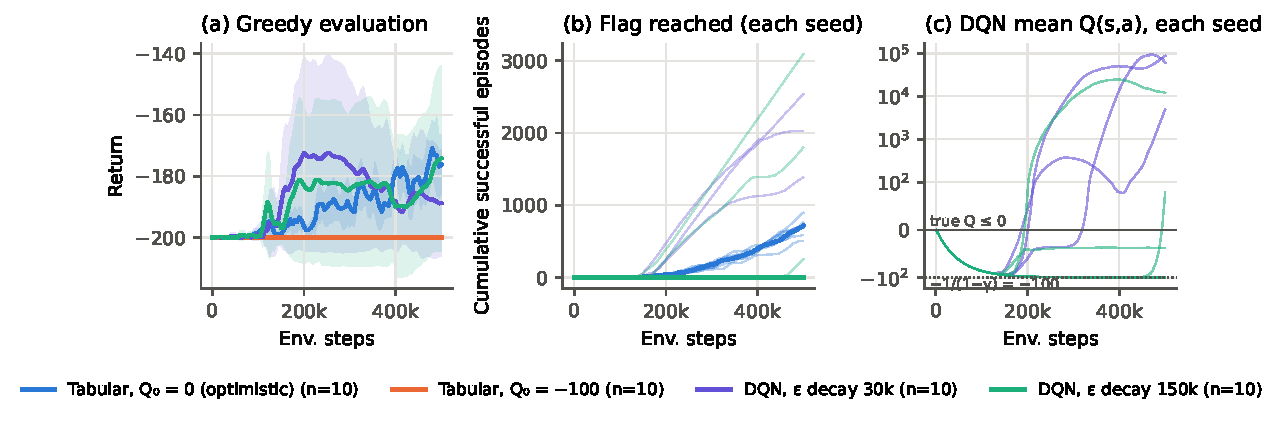
\includegraphics[width=0.98\textwidth]{t1_mountaincar.pdf}
\caption{MountainCar-v0, 500k steps, identical $\varepsilon$ schedule for all agents. (a) Greedy return
(mean $\pm$ 95\% CI). (b) Cumulative flag-reaching training episodes; thin lines are seeds, the thick line
is the median. (c) Mean $Q(s,a)$ on DQN training batches per seed (symmetric-log axis). Before the flag
every run sits at $-1/(1-\gamma)=-100$, and after it most runs diverge to impossible positive values.}
\label{fig:mc}
\end{figure*}

\tab{t1_mountaincar}

MountainCar pays $-1$ on every step, and an episode ends at the flag or after 200 steps. To isolate the
cause of failure, all four agents share the same $\varepsilon$ schedule ($1\!\to\!0.05$ over 30k steps,
or 150k for the second DQN). Fig.~\ref{fig:mc} and Table~\ref{tab:t1_mountaincar} summarize the result.

\paragraph{Optimism, not tabular-ness, is what explores.} With $Q_0=0$, every true value ($<0$) lies
below the initial estimate. Each visit lowers the tried action's value, so untried actions look better,
and the agent sweeps the state space systematically. It reached the flag on \emph{10/10} seeds (median
first success at 113k steps) and its greedy return improved to $-176\pm10$ (best $-148\pm6$). The
\emph{same} agent with $Q_0=-100=-1/(1-\gamma)$ has no optimism bonus and failed on \emph{all} 10 seeds,
with a greedy return of exactly $-200$ throughout. The decisive variable is the initialization, not the
function class.

\paragraph{Why DQN usually fails.} Until the first success, every transition in the buffer has $r=-1$,
so every target is $-1+\gamma\max Q$, which converges to $-1/(1-\gamma)=-100$ in every state. In the
14/20 DQN runs that never found the flag, the final mean $Q$ is $-99.4\pm0.1$ and the greedy return is
$-200$. The network has learned that ``all states are equally bad'': the value landscape is flat, so no
gradient points toward the goal. Exploration is left to $\varepsilon$-greedy dithering, which almost never
produces the $\sim$100 coordinated back-and-forth pushes needed to build momentum. A longer
$\varepsilon$ decay did not help (3/10 vs.\ 3/10 seeds reach the flag), because more \emph{undirected}
noise is not more exploration.

\paragraph{What happens when DQN does see the flag.} In 6/20 runs a lucky random trajectory reached the
flag. Those runs then learned better greedy policies than the table ($-138\pm38$), but their value
estimates \emph{diverged}. In MountainCar every true $Q$ is $\le 0$, yet after the first success four of
the six runs climbed above $+4{,}900$ (up to $9.6\cdot10^4$), one reached $+79$ and only one stayed below
zero. The pre-clip gradient norm rose from $\approx$0.4 to as much as $7.9\cdot10^3$. This is the
``deadly triad'' of function approximation, bootstrapping and off-policy updates
\citep[Sec.~11.3]{sutton2018}. The flag creates a sharp value cliff between $-1$ and $-100$ that the MLP
cannot represent locally. The error spreads to nearby states and is then amplified by the $\max$ in
every bootstrap target. The policy can stay reasonable because $\arg\max$ depends only on how the values
rank, not on their scale. A tabular update can never diverge like this, because each update moves only
its own cell toward its target. A unit test (\texttt{test\_dqn\_targets\_terminal\_and\_bootstrap})
confirms that terminal transitions use $y=r$ exactly, which rules out a terminal-handling bug.


\section{Tier 2: DQN ablations on LunarLander-v3}
\label{sec:t2}
\begin{figure*}[t]
\centering
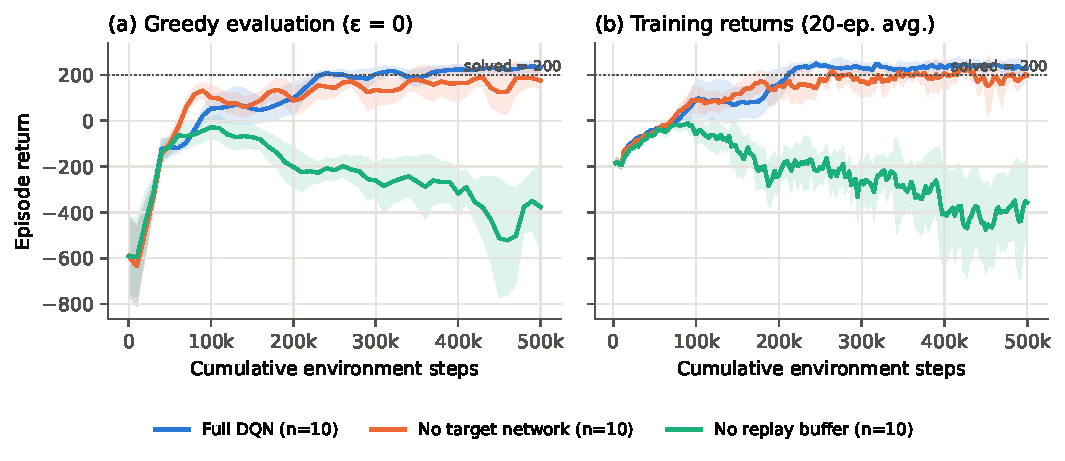
\includegraphics[width=0.92\textwidth]{t2_ablation.pdf}
\caption{LunarLander-v3 ablations, 500k steps, 10 seeds. Identical hyper-parameters except the removed
component.}
\label{fig:t2}
\end{figure*}

\tab{t2_lunarlander}

The full agent solves LunarLander on 10/10 seeds, with a final greedy return of $234\pm29$
(Table~\ref{tab:t2_lunarlander}, Fig.~\ref{fig:t2}). We then remove one stabilizer at a time and keep
every other hyper-parameter fixed.

\paragraph{No target network: learns, but cannot stay good.} Bootstrapping from the online network makes
the regression target move with every gradient step. Early learning is just as fast. The peak greedy
return matches the full agent ($275\pm7$ vs.\ $273\pm6$), and every seed reaches 200 at some point. But
the agent cannot hold its policy. All 10/10 seeds that reached $\ge$200 later fell below 0, against 2/10
for full DQN. The drop from peak to final is $99\pm35$ (full: $39\pm29$), and the final score is lower
($176\pm37$, Welch $p=0.014$). The TD loss stays higher throughout (Fig.~\ref{fig:diag}a): the network
keeps chasing a target that its own updates move. In this setting the target network buys
\emph{stability} rather than speed.

\paragraph{No replay buffer: never really learns.} Online DQN takes one gradient step per environment step
on the transition that just happened. Consecutive LunarLander states are almost identical, so the
mini-batches are strongly correlated and far from i.i.d. Each transition is also used once and
discarded. The agent improves briefly to a best of $149\pm28$, then degrades to a final $-376\pm188$
(Welch $p<10^{-4}$ vs.\ full), and only 2/10 seeds ever touch 200. Its diagnostics show the failure.
The mean batch $Q$ inflates to $257$, $5.9\times$ the full agent's, while its policy is much worse,
which is clear overestimation. Its gradient norms reach $\sim$300 before clipping, against $\sim$20
for full DQN, and its loss never comes down (Fig.~\ref{fig:diag}). Each update fits the current stretch
of trajectory and overwrites the rest (catastrophic interference). Its CPU cost is also the highest
(24 vs.\ 10 min per run), because it updates on every step instead of every fourth.

\begin{figure*}[t]
\centering
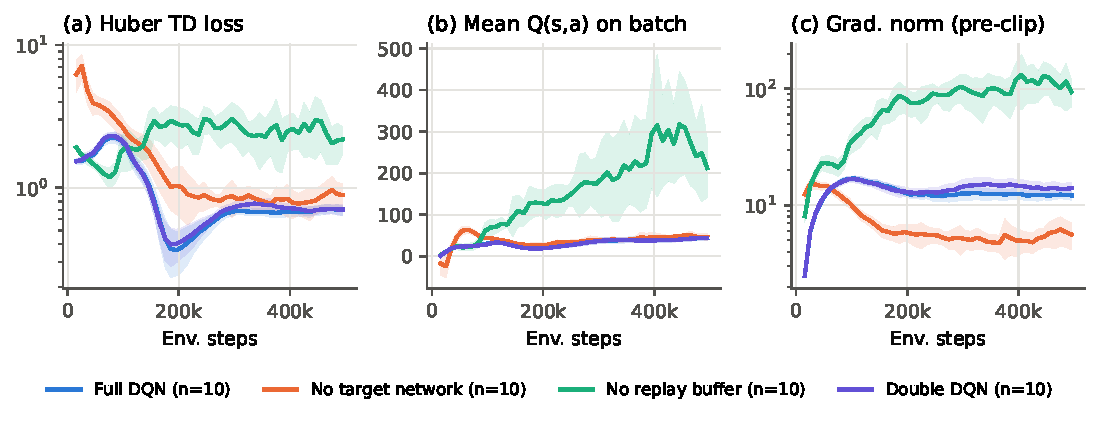
\includegraphics[width=0.92\textwidth]{t2_diagnostics.pdf}
\caption{Training diagnostics (10k-step block averages): Huber TD loss (log), mean $Q(s,a)$ on training
batches, and pre-clip gradient norm (log).}
\label{fig:diag}
\end{figure*}

\paragraph{Double and Dueling DQN (Tier 3B).} Neither extension changed the outcome measurably at this
scale. Final returns were $234\pm29$ (Double) and $238\pm33$ (Dueling) against $234\pm29$ for full DQN
($p=0.98$ and $0.82$), and all three solved 10/10 seeds. Double DQN also left the $Q$ level unchanged
($43.2$ vs.\ $43.4$). With 4 actions, a target network refreshed every 1{,}000 steps, and a Huber loss,
the overestimation that Double DQN removes is already small. Its benefit reported by
\citet{vanhasselt2016} was on Atari, with 18 actions and much noisier value estimates. We report this
as a null result rather than tuning until a difference appears.

\paragraph{Hyper-parameter study.} We varied two parameters one at a time around the default, with three
values each and 5 seeds (seeds 0--4, the same seeds for every row; Fig.~\ref{fig:hp},
Table~\ref{tab:t2_hparams}). Only a too-small learning rate hurts significantly. With $\text{lr}=10^{-4}$ the
agent learns too slowly for the 500k budget: its final score is $106\pm117$ against $258\pm17$ (Welch
$p=0.022$), and only 3/5 seeds ever reach 200. A larger rate ($2\cdot10^{-3}$) reaches 200 sooner (118k vs.\
200k steps) but ends lower and more variable ($234\pm48$, $p=0.26$). The target-update period behaves the
same way. Copying every 250 steps learns faster (146k) and forgets more (drop $53$ vs.\ $15$). Copying
every 4{,}000 steps learns slower (252k) but is steadier than 250. Neither final score differs
significantly from the default ($p=0.22$ and $0.27$). Both parameters therefore trade learning speed
against stability, and removing the target network (Sec.~\ref{sec:t2}) is the extreme case of a period of one step.

\begin{figure*}[t]
\centering
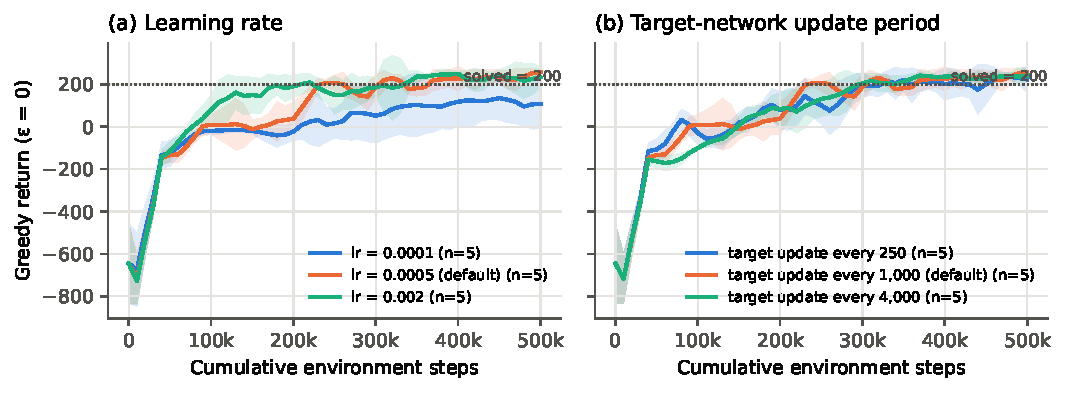
\includegraphics[width=0.92\textwidth]{t2_hparams.pdf}
\caption{LunarLander-v3 hyper-parameter study (greedy evaluation, 5 seeds, 95\% CI). One parameter is
varied at a time, and all other settings are as in Full DQN.}
\label{fig:hp}
\end{figure*}

\tab{t2_hparams}

\paragraph{Official 100-episode evaluation.} The thresholds are defined over 100 episodes, whereas our
curves use 10 episodes per checkpoint and count a seed as solved when \emph{any} checkpoint reaches the
threshold. We therefore reloaded the \emph{final} weights of every run and played 100 greedy episodes from
held-out start states (\texttt{experiments/eval100.py}, Table~\ref{tab:t_final100_main}). Full DQN on
LunarLander passes (mean $227$; 7/10 seeds $\ge200$). On CartPole, only 4/10 tabular (10 bins) and 5/10 DQN
($\varepsilon$ decay 5k) final policies average $\ge475$. Every seed had reached 475 at some checkpoint, so
this is the forgetting of Sec.~\ref{sec:cp} measured on the final weights. On MountainCar, the optimistic
table reaches the flag in 64\% of the evaluation episodes (DQN: 19\%), taking $\approx$160 steps when it
does, so it falls short of the $-110$ threshold (0/10 seeds). We therefore claim that it \emph{finds the goal}, not that it solves the task.

\tab{t_final100_main}

\begin{figure}[t]
\centering
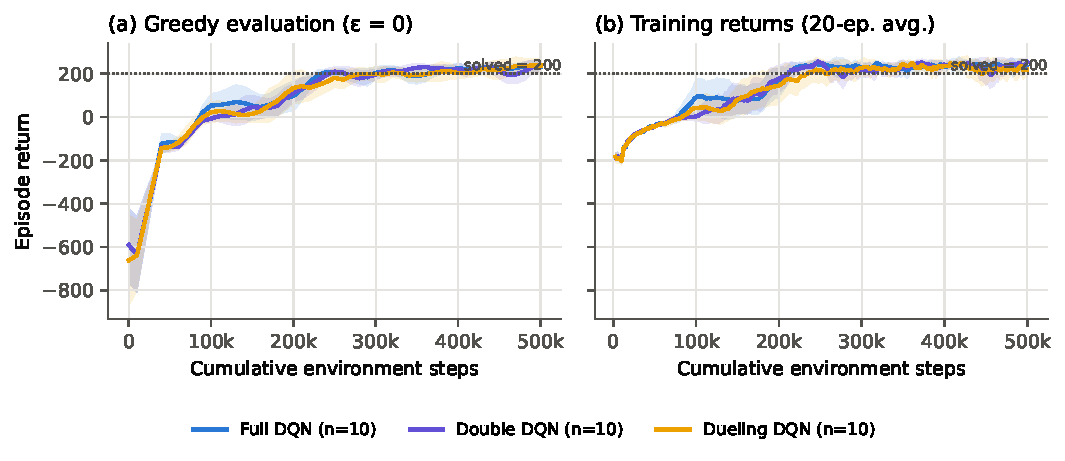
\includegraphics[width=\columnwidth]{t2_extensions.pdf}
\caption{Double and Dueling DQN vs.\ the full agent: indistinguishable within the 95\% CIs.}
\label{fig:ext}
\end{figure}

\section{Compute cost}
The full study comprises 170 runs and 22.3 CPU-hours (one thread per run). On the reference laptop, per
run, a 1M-step CartPole table takes $\approx$100\,s, a 200k-step CartPole DQN $\approx$450\,s, and a
500k-step LunarLander DQN $\approx$10 minutes (24 without replay). The deep agents account for most of
the budget even though they use 5$\times$ fewer environment steps on CartPole. This is the
sample-efficiency vs.\ compute trade-off of Sec.~\ref{sec:cp}, made concrete.


\section{Analysis: limits of tabular RL and DQN in complex environments}
\label{sec:theory}
\paragraph{Discretizing continuous actions.} DQN needs a finite action set, because its output layer has
one node per action and acting requires $\max_a$. HalfCheetah has a 6-D continuous action in $[-1,1]^6$.
With only 5 levels per joint, the joint action set has $5^6=15{,}625$ elements. The output layer grows
accordingly, $\max_a$ must scan all of them, and, most importantly, each $Q(s,a)$ is learned from the
few samples in which that \emph{exact} combination was tried. $\varepsilon$-greedy exploration over
15{,}625 arms is hopeless, and the coarse grid still cannot express smooth torques. Ant (8-D) would need
$5^8\approx3.9\cdot10^5$ actions. The action space itself suffers the curse of dimensionality.

\paragraph{Discretizing continuous states.} The table needs $k^{d}$ cells. HalfCheetah's 17-D observation
with $k=10$ gives $10^{17}$ cells per action. That is roughly $8\cdot10^{17}$ bytes per action for
\texttt{float64}, far beyond any memory. Even if memory were free, filling each cell even once would
take more interactions than could ever be collected. Our CartPole results already show the trend in
4-D: going from 6 to 20 bins multiplied the table by 123, and the fraction of states ever visited fell
from 39\% to 4.6\%. Coarse coding and tile coding \citep[Ch.~9]{sutton2018} soften this by letting
states share features, but the number of tiles still grows exponentially with $d$.

\paragraph{Algorithms for continuous control.} The remedy is to parameterize the \emph{policy} directly
and use a learned critic (actor--critic methods), which avoids $\max_a$ over an enumerated set.
\textbf{PPO} \citep{schulman2017} is on-policy. Its actor outputs the mean (and log-std) of a Gaussian
over actions, and its clipped surrogate objective limits the size of each policy update.
\textbf{SAC} \citep{haarnoja2018} is off-policy and stochastic. It maximizes return plus policy entropy,
which gives strong, automatically tuned exploration and good sample efficiency on MuJoCo.
\textbf{TD3} \citep{fujimoto2018} is off-policy and deterministic. Its actor outputs the action vector,
and twin critics with a $\min$, delayed actor updates and target-policy smoothing counter the same
$\max$-overestimation bias that Double DQN addresses in the discrete case.

\paragraph{Why tables fail on pixels.} An Atari frame is $210\times160$ RGB. Even downsampled to
$84\times84$ grayscale with 256 intensities, the number of distinct observations is
$256^{7056}\approx10^{16{,}992}$. A table learns only about states it has visited \emph{exactly}, and the
chance of seeing the same frame twice (outside a few reset states) is essentially zero, so no update
would ever be reused. What makes Atari tractable is \emph{generalization}: a convolutional network maps
visually similar frames to similar features, so experience transfers between states that are never
identical. That is the same mechanism that gave DQN its $\approx$7$\times$ sample-efficiency advantage on
CartPole, applied at a far larger scale \citep{mnih2015}.

\section{Conclusion}
Tabular Q-learning and DQN fail and succeed for identifiable reasons. On CartPole, DQN's ability to
generalize between states made it $\approx$7$\times$ more sample-efficient, but it cost 23$\times$ more
CPU per step, so the table was cheaper in compute. DQN also forgot solved policies, which only shows
up when evaluation is tracked \emph{during} training. The table's performance depends on a precision/data
trade-off in the discretization. MountainCar showed that what explores is optimism, not the function
class. A pessimistic table fails exactly like DQN. DQN fails because a reward that is $-1$ everywhere
flattens its value function, and when it does reach the flag, its estimates can diverge (the deadly
triad). On LunarLander, the target network was needed to \emph{keep} a good policy and the replay
buffer to \emph{find} one at all. Double and Dueling heads gave no measurable gain at this scale.
Finally, none of these methods transfers to continuous control or pixel observations without replacing
enumeration by generalization (Sec.~\ref{sec:theory}).

\section*{AI-use statement}
We used Claude (Anthropic), through the Claude Code assistant, for code generation, debugging, and
writing support. This included drafting experiment scripts and helpers, checking the repository against
the project requirements, and editing this report. Every number in the text, tables and figures is produced
by our own scripts (\texttt{analysis.py}, \texttt{experiments/*.py}) from the logged runs in
\texttt{results/}. No result was taken from the assistant without being regenerated by that code. Both authors reviewed the AI-generated code, and
we take responsibility for all of it. The most important prompts are listed in Appendix~\ref{app:prompts}.



\bibliographystyle{plainnat}
\bibliography{references}

\appendix
\section{Most important AI prompts}
\label{app:prompts}
\small
% Add here the key prompts you used earlier in the project (e.g. when building agents/dqn.py,
% the discretizer, the runner and the report), in the same format.
\begin{enumerate}
\item \emph{Requirements check.} We pasted the full project statement and the repository link and asked:
``Is everything here? We are a group of 2.'' The assistant listed the missing items (Tier 2
hyper-parameter study, agent videos, AI-use statement, 100-episode evaluation), and we asked it to implement them.
\item \emph{Tier 2 hyper-parameter study.} Asked to add a one-at-a-time study of the learning rate and the
target-update period around the default LunarLander configuration, reusing the existing runner, seeds
and table format (\texttt{experiments/tier2\_hparams.py}).
\item \emph{Final evaluation and videos.} Asked for a script that reloads the final weights of every run and
plays 100 greedy episodes against the official thresholds (\texttt{experiments/eval100.py}), and for
GIFs of a representative (median) seed per agent (\texttt{experiments/make\_gifs.py}).
\end{enumerate}
\end{document}
